\documentclass{article}
\usepackage[margin=1in]{geometry}
\usepackage{amsmath, amssymb, amsthm}
\usepackage{enumitem}

% colored links
\usepackage{hyperref}
\hypersetup{
    colorlinks=true,
    linkcolor=blue,
    filecolor=magenta,      
    urlcolor=magenta,
    }


% Inputting Python code
\usepackage[dvipsnames]{xcolor}
\definecolor{textblue}{rgb}{.2,.2,.7}
\definecolor{textred}{rgb}{0.54,0,0}
\definecolor{textgreen}{rgb}{0,0.43,0}
\usepackage{upquote}
\usepackage{listings}
\lstset{
    language=Python, 
    tabsize=4,
    basicstyle={\ttfamily},
    keywordstyle=\color{textblue},
    commentstyle=\color{textgreen},
    stringstyle=\color{textred},
    frame=none,
    columns=fullflexible,
    keepspaces=true,
    showstringspaces=false,
    xleftmargin=-15mm, % manual adjustment, figure out permanent solution
}

\newcommand{\gray}[1]{\textcolor{gray}{#1}}

%Creating algorithms
\usepackage{algorithm}
\usepackage[noend]{algpseudocode}

\usepackage{tcolorbox}
\tcbuselibrary{skins,hooks}
\usetikzlibrary{shadows}
\usepackage{lipsum}

%Images
\usepackage{graphicx}
    \usepackage{subcaption}
    \usepackage{float}
    % \usepackage[labelsep=period]{caption}

    
%Creating Figures
\usepackage{tikz}
\usetikzlibrary{calc, math, matrix, graphs, positioning}


% the settings of tikz is used for the optimization of the graphs  
\usetikzlibrary{shapes, arrows, calc, arrows.meta, fit, positioning} % these are the parameters passed to the library to create the node graphs  
\tikzset{  
    -Latex,auto,node distance =1.1 cm and 1.1 cm, thick,% node distance is the distance between one node to other, where 1.5cm is the length of the edge between the nodes  
    state/.style ={ellipse, draw, minimum width = 0.9 cm}, % the minimum width is the width of the ellipse, which is the size of the shape of vertex in the node graph  
    point/.style = {circle, draw, inner sep=0.18cm, fill, node contents={}},  
    el/.style = {inner sep=2.5pt, align=right, sloped}  
}  

%Formatting and Spacing
\setitemize[1]{noitemsep, parsep = 5pt, topsep = 5pt}
\setenumerate[1]{label = (\alph*), parsep = 1pt, topsep = 5pt}
\setlength\parindent{0pt}
\linespread{1.1}

% title
\title{\vspace{-1cm}CS 2051: Honors Discrete Mathematics \\Spring 2023 Homework 5 Supplement}
\author{Sarthak Mohanty }
\date{}

\begin{document}

\maketitle

\section*{Overview}

   \qquad Traditionally, computer software has been written for serial computation: instructions corresponding to a tasks are executed on one processing unit at a time. However, nowadays many computational tasks consist of many elementary operations, some of which have to be computed sequentially, while others can be computed in parallel.

    \vspace{2mm}
    \qquad In a distributed or high performance computing course, one of the first things you may learn is \href{https://en.wikipedia.org/wiki/Amdahls_law}{Amdahl’s law}, which gives a quantitative measure of the speedup $S$ -- i.e., how much faster the task can be performed by using $n$ parallel processors: $$S = \frac{1}{1 - p + \frac{p}{n}}.$$ Here, $p$ is the proportion of operations that can be performed in parallel.


    \vspace{2mm}
    \qquad However, it is not typically the case that we can classify operations simply as “parallel” or “sequential.” Instead, a task might consist of several sub-tasks, some of which need to be completed before others are started. Optimally scheduling these tasks is much trickier, and is currently an area of \href{https://www.cs.umd.edu/~samir/DCscheduling18/slides/Janardhan Kulkarni.pdf}{active research}. However, with the right mathematical foundations, we can at least start to understand the complexity of task scheduling, and develop efficient strategies for tackling ``easy" versions of these problems.

    \vspace{2mm}
    \qquad In this supplement, you learn about a generalized form of functions known as \textbf{relations}, and explore the connection between functions and relations. You'll then learn about two important types of relations, including \textbf{equivalence relations} and \textbf{partial orders}. Finally, we'll explore some of the applications of these concepts, including a return to our original problem of multi-processor scheduling.

\section*{Part 1: Generalizing Functions with Relations (10 pts)}

    This week, you learned about functions. We (informally) defined them as a well-defined mapping between two sets. However, what about mappings that are not well-defined? Is there no way to represent these? As a matter of fact, there is!
    
    \vspace{3mm}
    \textbf{Definition.} a \textit{relation} $\mathcal{R}$ over sets $A, B$ is a subset of $A \times B$. The notation $a\mathcal{R}b$ or $a \sim b$ is often used to denote that $(a, b) \in \mathcal{R}$.

    \subsection*{Easy Examples}
    
    The following are all valid relations on $A \times A$, where $A = \{1, 2, 3, 4\}$
    \begin{itemize}
        \item $\mathcal{R}_1 = \{(a, b) \mid a \le b)\}$
        \item $\mathcal{R}_2 = \{(a, b) \mid a = b)\}$
        \item $\mathcal{R}_3 = \{(a, b) \mid a+b \le 2023)\}$
        \item $\mathcal{R}_4 = \{(a, b) \mid a \text{ divides } b\}$
    \end{itemize}

    \subsection*{Another Example: Functions}
    Functions are also an example of relations. Specifically, a function is any relation $\mathcal{R}: A \rightarrow B$ with the property that for any $x$ there is exactly one $y$ such that $x\mathcal{R}y$.
    
    
\subsection*{Properties of A Relation $\mathcal{R} \colon A \rightarrow A$}

    \begin{enumerate}[align=left]
        \item [\textbf{Reflexitivty}] $\mathcal{R}$ is \textit{reflexive} if 

        $(\forall a \in A)(a\mathcal{R}a)$

        ``Everyone has slept with themselves"
        \item [\textbf{Symmetry}] $\mathcal{R}$ is \textit{symmetric} if 

        $(\forall a, b \in A)(a\mathcal{R}b \iff b\mathcal{R}a)$

        ``If $a$ slept with $b$, then $b$ slept with $a$"

        \item [\textbf{Antisymmetry}] $\mathcal{R}$ is \textit{symmetric} if 

        $(\forall a, b\in A)(a\mathcal{R}b \wedge b\mathcal{R}a \rightarrow a=b)$

        ``No pair of distinct people have slept with each other"

        \item [\textbf{Transitivity}] $\mathcal{R}$ is \textit{transitive} if 

        $(\forall a, b, c\in A)(a\mathcal{R}b \wedge b\mathcal{R}c \rightarrow a\mathcal{R}c)$

        ``If $a$ slept with $b$ and $b$ slept with $c$, then $a$ slept with $c$ too."
    \end{enumerate}

    When a relation is reflexive, antisymmetric, and transitive, we call it a \textit{partial order}. When a relation is reflexive, symmetric, and transitive, we call it a \textit{equivalence relation}.

    \vspace{3mm}
    \begin{tcolorbox}[colback=yellow!30]
        \textbf{In this part, you'll implement the following (one-line) functions:}
        \begin{itemize}
            \item \lstinline{isPartialOrder(elements, relation)}: This function takes in a relation (represented as a set of tuples) and returns whether or not the relation (taken over the set of elements) is a valid partial order.
            \item \lstinline{isEquivalenceRelation(elements, relation)}: This function takes in the same arguments are before, but this time returns whether or not the relation is a valid equivalence relation.
        \end{itemize}
        You may also implement the following (self-explanatory) helper methods to assist in your solution, as long as they are also one-liners:
        \begin{itemize}
            \item \lstinline{isReflexive(elements, relation)}
            \item \lstinline{isSymmetric(elements, relation)}
            \item \lstinline{isAntisymmetric(elements, relation)}
            \item \lstinline{isTransitive(elements, relation)}
        \end{itemize}
        \textbf{}

        \vspace{2mm}
        A few tips:
        \begin{itemize}
            \item The \lstinline{all(iterable)} method returns true if all elements of the iterable are true (or if the iterable is empty)
            \item Now may also be a good time to learn (if you haven't already) about \href{https://docs.python.org/3/tutorial/datastructures.html#list-comprehensions}{list comprehension}.
        \end{itemize}
    \end{tcolorbox}


\section*{Part 2: Partitioning with Equivalence Relations (10 pts)}
    In the world of computer science, there are two main applications for relations: partitioning and scheduling. In this part, we'll cover partitioning, which is essentially just a reframing of our knowledge about equivalence relations.

    \vspace{2mm}
    \textbf{Definition}: Given some relation $\mathcal{R}$ over the set $A$, the \textit{equivalence class} of an element $x \in A$ is $[x] = \{y : x \mathcal{R} y\}$.

    \vspace{2mm}

    Equivalence classes are useful because they all us to ``break apart" any set into disjoint, nonempty subsets. The following theorem formalizes this idea.

    \begin{tcolorbox}
        \textbf{Theorem}: The equivalence classes of an equivalence relation on a set $A$ \textit{partition} $A$ into a collection of disjoint, nonempty subsets $A_{1}, A_{2}, \dots, A_{n}$ such that (and this is the important part) $\bigcup _{i = 1}^{n} = A$.
    \end{tcolorbox}
    
    \vspace{2mm}
    Ok, so this fact is cool and all, but what's the point? Well, if we have say a million elements in a set, but only three equivalence classes, we need only consider the three classes to understand the properties of the entire set. This is where the concept of \textit{canonical forms} comes in, which refers to the standard representation of a set in terms of its equivalence classes, making it easier to analyze and manipulate.
    
    \vspace{2mm}If you're not convinced already, the following examples should illuminate the power of equivalence classes.

    \subsection*{Example: Congruence Relations}
        Our first example delves into basic number theory. Informally, define the relation $a\mathcal{R}_{n}b$ over $\mathbb{Z} \times \mathbb{Z}$ if $a$ and $b$ have the same remainder when divided by some number $n$. We usually denote this using $$a \equiv b \pmod{n}.$$ For example, $-10$ and $15$ are related under $\mathcal{R}_{5}$, $$-10 \equiv 15 \pmod{5},$$ since $-10 - 15 = -25$ is a multiple of $5$, or equivalently since both $-10$ and $15$ have the same remainder $0$ when divided by $5$.
        
        \vspace{2mm}
        All such relations $\mathcal{R}_{n}$ are equivalence relations. Thus, they partition the set of integers into $n$ disjoint, nonempty equivalence classes. For example, the relation $\mathcal{R}_{3}$ partitions the integers as
        \begin{gather*}
            \{\dots, -7, -4, -1, 2, 5, 8, \dots\} \\
            \{\dots, -8, -5, -2, 1, 4, 7, \dots\} \\
            \{\dots, -9, -6, -3, 0, 3, 6, \dots\}
        \end{gather*}
        The canonical forms for each of these sets are $2$, $1$, and $0$ respectively. An illustration for the congruency classes in general is shown in Figure (\ref{fig:congruency_classes}).

        \begin{figure}[htbp]
            \centering
            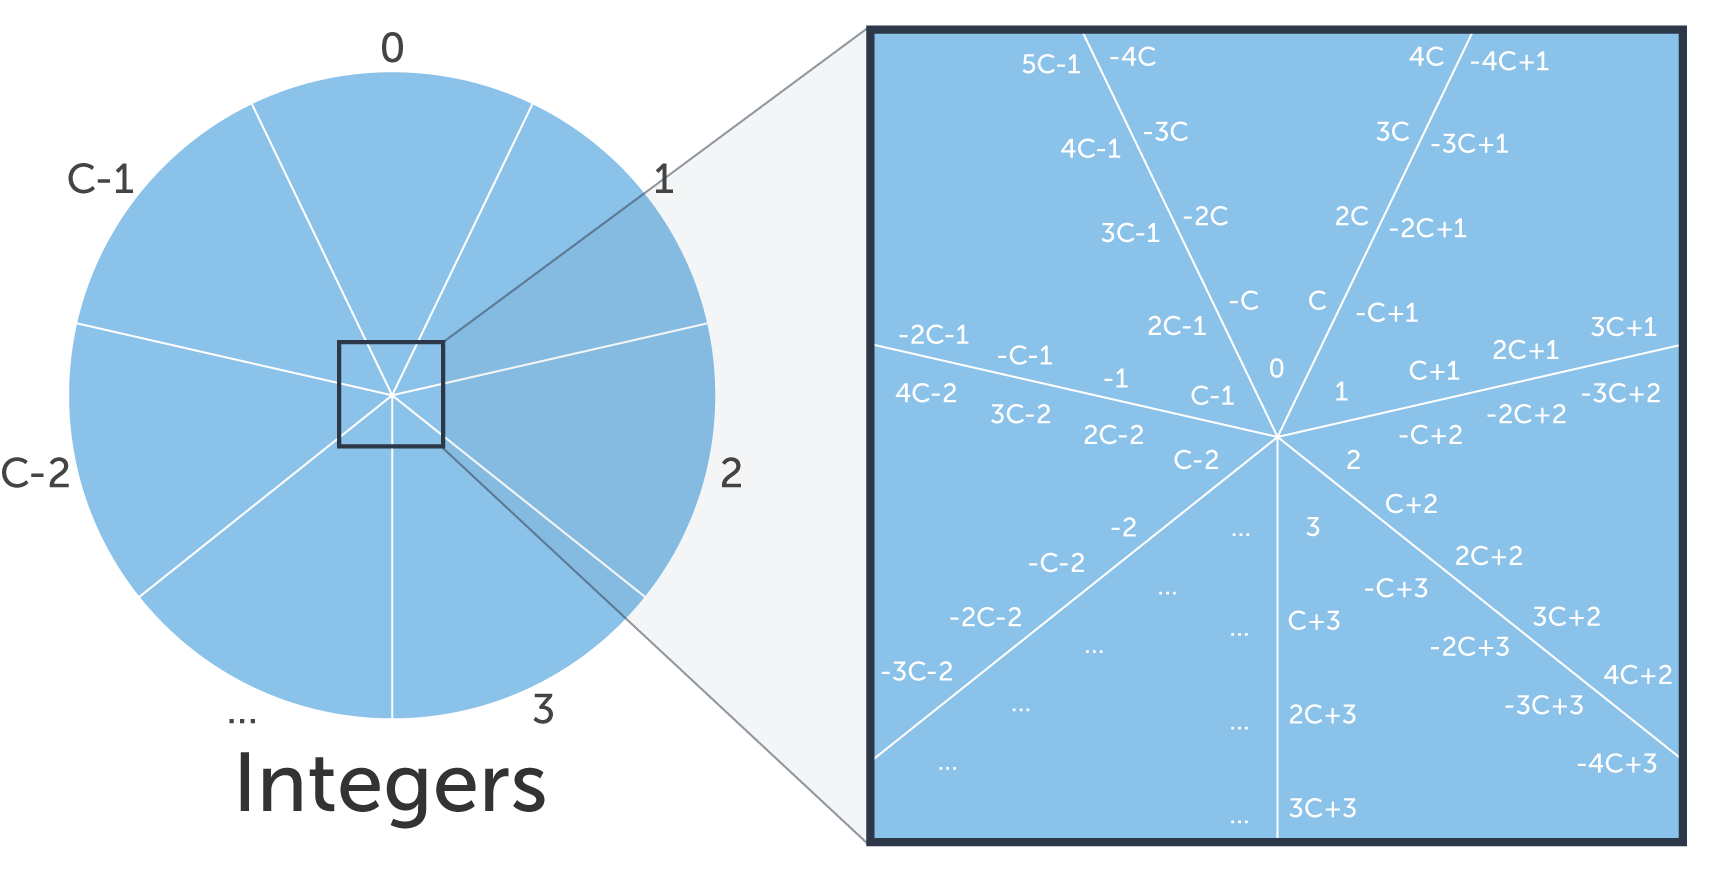
\includegraphics[scale = .4]{sp23/hw-supplements/hw5-supp/images/congruence_classes.png}
            \caption{The partition of the set of integers over the congruence relation $\mathcal{R}_{C}$.}
            \label{fig:congruency_classes}
        \end{figure}
        


    \subsection*{Example: Vector Spaces}
        One of the most prominent uses of equivalence classes is in linear algebra. After all, it's very difficult to determine when two vector spaces or matrices are functionally ``identical". 

        \vspace{3mm}
        If you've taken an introductory linear algebra course, you learned about Gauss's Method to solve a system of equations. In essence, it worked by starting with a matrix and deriving a sequence of other matrices, each \textit{row equivalent} to each other. It turns out that row equivalence is an equivalence relation, and partitions the set of all matrices into corresponding classes, as shown in Figure (\ref{fig:1}).

        \vspace{3mm}
        We can generalize this one step further with a relation known as \textit{matrix equivalence}. Two matrices are matrix equivalent if they be derived using a combination of row operations \textit{and} column operations. Matrix equivalence classes are also characterized by rank: two same-sized matrices are matrix equivalent if and only if they have the same rank.
        
        \vspace{2mm}
        Looking at these definitions for matrix equivalence, you may notice they are analogous to the definition of matrix similarity you learned in your linear algebra course. This is no coincidence! In fact, matrix similarity is itself an equivalence relation, and is a special case of matrix equivalence! (see Figure (\ref*{fig:3}) for an illustration)

        \vspace{3mm}
         The canonical forms for row equivalence are the Reduced Echelon form matrices, which you may already be familiar with. Meanwhile, the canonical forms for matrix similarity are known as Jordan Normal forms. The canonical forms for matrix equivalence are a bit more complicated, but an example is shown in Figure (\ref*{fig:2}).
        
        \begin{figure}[H]
            \centering
            \captionsetup{width=.6\linewidth}
            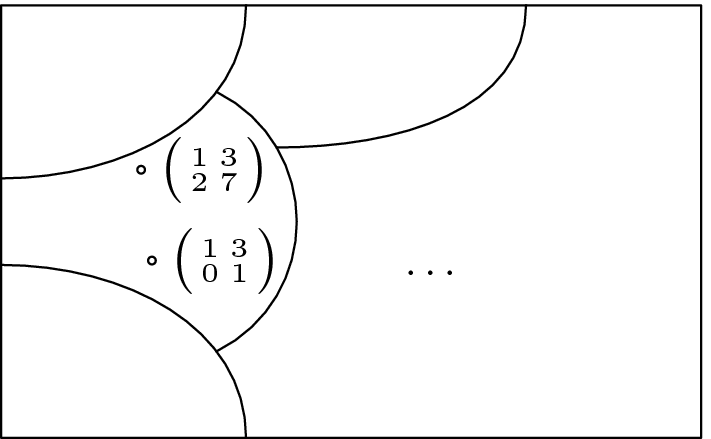
\includegraphics[scale = .3]{sp23/hw-supplements/hw5-supp/images/linalg_reduced_echelon_form_equiv_classes.png}
            \caption{The two matrices above can be row reduced to each other. Thus under row equivalence, they are partitioned into the same equivalence class.}
            \label{fig:1}
        \end{figure}

        \begin{figure}[H]
            \centering
            \captionsetup{width=.6\linewidth}
            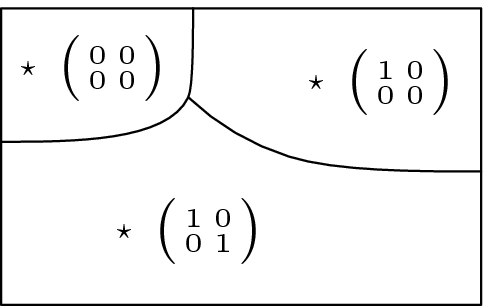
\includegraphics[scale = .4]{sp23/hw-supplements/hw5-supp/images/linalg_2by2_rank_equivalence_classes.png}
            \caption{The canonical forms of each of the equivalence classes corresponding to matrix equivalence taken over the set of $2 \times 2$ matrices. The matrices have rank $0$, $1$, and $2$ respectively.}
            \label{fig:2}
        \end{figure}

        \begin{figure}[H]
            \centering
            \begin{subfigure}{0.45\textwidth}
                \centering
                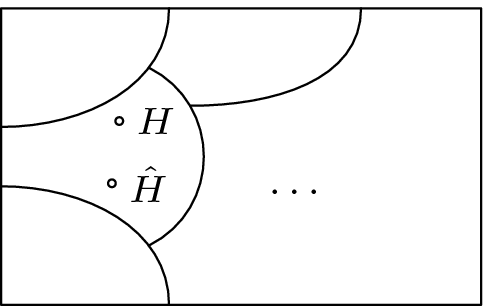
\includegraphics[scale = .35]{sp23/hw-supplements/hw5-supp/images/linalg_matrix_equivalence_classes.png}
                \caption{The equivalence classes of matrix equivalence.}
            \end{subfigure}
            \begin{subfigure}{0.45\textwidth}
                \centering
                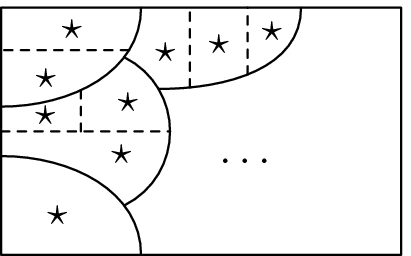
\includegraphics[scale = .41]{sp23/hw-supplements/hw5-supp/images/linalg_matrix_similarity_equiv_classes.png}
                \caption{The equivalence classes of matrix similarity.}
            \end{subfigure}
            \caption{Matrices $H$ and $\hat{H}$ are matrix equivalent, but they may not be similar to each other.}
            \label{fig:3}
        \end{figure}

    \vspace{3mm}
    \begin{tcolorbox}[colback=yellow!30]
        \textbf{In this part, you'll implement the following function:}
        \begin{itemize}
            \item \lstinline{partition(elements, relation)}: This function takes a equivalence relation (this time represented as a boolean function), and returns a partition of the elements into equivalence classes. For example, given the congruence relation described above, the function should return
        \begin{lstlisting}[belowskip=-10pt]
            >>> partition([i for i in range(-8, 8)], lambda x, y: (x - y) % 3 == 0)
            [{-6, -3, 0, 3, 6}, {-8, -5, -2, 1, 4, 7}, {-7, -4, -1, 2, 5}]
        \end{lstlisting}

        \end{itemize}

        Tip: iterating over sets is difficult. Try casting.
    \end{tcolorbox}

    % idea: quotient graph https://networkx.org/documentation/stable/_modules/networkx/algorithms/minors/contraction.html#equivalence_classes

\section*{Part 3: Single-Processor Task Scheduling (10 pts)}

    We now delve into partial orderings, or ``posets". We'll cover a nice \textit{graph}ical representation of posets, and then cover their applications in the context of task scheduling. 
    
    \subsection*{Dependency Graphs}
    
    To start, let's consider the following story. 

    \begin{tcolorbox}[colback=red!20]
        You're a recently admitted CS major at Georgia Tech. To save money, you're trying to graduate as early as possible.  You have a lot of courses you can take, but you're not sure which ones to take when. Furthermore, many of the courses are dependent upon completion of other courses (for example, CS 1332 requires CS 1331, which in turn requires CS 1301). How long will it take for you to graduate?
    \end{tcolorbox}

    Let $\mathcal{R}$ be a relation over the set of courses $A$, where $a \mathcal{R} b$ iff $a$ is a prerequisite to take $b$. We can use this relation to help model some sample graduation requirements by creating a \textit{dependency list} as follows:
    $$\mathcal{R} = 
    \left\{
    \begin{array}{ccc}
        (1301, 1331), & \gray{(1301, 1301)}, & \gray{(1301, 1332),} \\
        (1331, 1332), & \gray{(1331, 1331)}, & \gray{(1301, 4641),} \\
        (2051, 3511), & \gray{(1332, 1332),} & \gray{(1301, 3600),} \\
        (1332, 3511), & \gray{(2051, 2051),} & \gray{(1301, 3511),} \\
        (1332, 3600), & \gray{(4641, 4641),} & \gray{(1331, 4641),} \\
        (1332, 4641), & \gray{(3511, 3511),} & \gray{(1331, 3600),} \\
        (1301, 1301), & \gray{(3511, 3600),} & \gray{(1331, 3511)} \\
    \end{array}
    \right\}$$
    (the greyed-out tuples are added to ensure the relation is a partial order). However, this doesn't really provide us with much intuition. Since this relation is a partial order, we can alternatively visualize it using something called a \textbf{dependency graph}, an example of which is shown in Figure (\ref{fig:dependency_graph}). While programs can only understand dependency lists, you may find the graphical representation useful for testing and debugging your implementations for the remaining parts.
    
    \begin{figure}[htbp]
            \centering
            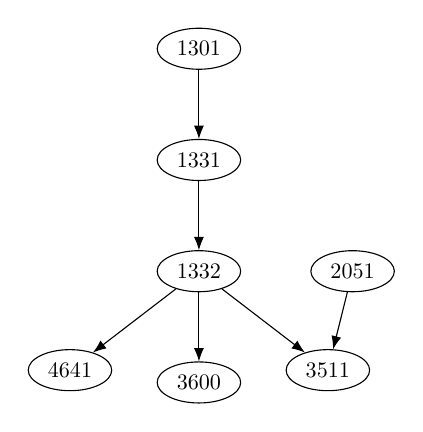
\begin{tikzpicture}[scale = 0.8, transform shape]  
                \node[state] (1301) at (0,0) {1301}; % here, state signifies that the shape of the node will be the shape declared in the above state/.style command.  
                \node[state] (1331) [below =of 1301] {1331};  
                \node[state] (1332) [below =of 1331] {1332};
                \node[state] (2051) [right =of 1332] {2051};  
                \node[state] (4641) [below left =of 1332] {4641};  
                \node[state] (3600) [below =of 1332] {3600};  
                \node[state] (3511) [below right =of 1332] {3511};  
                \path (1301) edge (1331); % it is the path of the edge from one node to another  
                \path (1331) edge (1332);
                \path (1332) edge (4641);
                \path (1332) edge (3600);
                \path (1332) edge (3511);
                \path (2051) edge (3511);
            \end{tikzpicture} 
            \caption{A dependency graph corresponding to some graduation requirements}
            \label{fig:dependency_graph}
        \end{figure}

    \subsection*{Task Scheduling}
    
    Using the formalism of posets, we can also define the problem of computing an optimal schedule.

    \vspace{3mm} Assume that some task $T$ can be decomposed into sub-tasks $T = \{T_{1}, T_{2}, \dots, T_{n}\}$. In general, we can encode the relationships between the various $T_{i}$ as a poset, where $T_{i} \prec T_{j}$ if (sub)task $T_{i}$ needs to be performed before $T_{j}$. \textbf{Assume each task $T_{i}$ takes 1 unit of time to complete.} Given $k$ processors $P_{1}$, $P_{2}$, \dots, $P_{k}$ a \textbf{schedule} for $T$ assigns each sub-task $T_{i}$ a processor $P_{j}$ as well as a time $t_{i}$ at which $P_{j}$ should start task $T_{i}$. Observe that if a processor starts $T_{i}$ at times $t_{i}$, then the task will complete at time $t_{i} + 1$. A schedule is \textbf{feasible} if:
    \begin{enumerate}[label = \arabic*]
        \item no single processor is performing multiple tasks at the same time (i.e., if a processor is assigned $T_{i}$ and $T_{j}$ at times $i, j$, then $i \ne j$) and
        \item for every pair of tasks $T_{i}$ and $T_{j}$ with $T_{i} \prec T_{j}$, task $T_{j}$ is scheduled to start some time after (or at the same time) $T_{i}$ completes. (i.e.\ $T_{i} \prec T_{j} \Rightarrow t_{j} > t_{i}$)
    \end{enumerate}
    The \textbf{latency} of a schedule is the total time between when the first task is scheduled to when the last task completes. Our goal is to find a schedule with the smallest latency.

    \subsection*{Topological Sorting}
    If we have only one processor, then constructing an algorithm to do this is fairly simple. Just schedule all the elements one by one in an order such that no element depends on any of the elements scheduled after it. This is also known as a \textit{topological sort}.

    \vspace{3mm}
    We present a common algorithm for finding the topological sort below, known as Kahn's algorithm. (Note: the pseudocode refers to \textit{minimal elements}. These are simply all elements $v$ such that there is no other element $u$ such that $(u, v) \in \mathcal{R}$.)

    \begin{algorithm}
        \caption{\textsc{KahnsAlgorithm}$(elements, poset)$}\label{alg:cap}
        \label{alg:topological_sort}
        \begin{algorithmic}
            \State $T = \emptyset$
            \State $S = $ all minimal elements in $poset$
            \While{$S \ne \emptyset$}
                \State $u = $ an element in $S$
                \State $S = S - \{u\}$
                \State $T = T \cup \{u\}$
                \State $uv\_dependencies = \{(u, v) : v \in elements \text{ and }(u, v) \in poset\}$
                \For{each $(u, v)$ in $uv\_dependencies$}
                    \If {$v$ is minimal} insert $v$ in $S$ \EndIf
                \EndFor
            \EndWhile
            \State \Return{T}
        \end{algorithmic}
    \end{algorithm}
    
    \begin{tcolorbox}[colback=yellow!30]
        \textbf{In this part, you'll implement the following function:}
        \begin{itemize}
            \item 
        \lstinline{topological_sort(elements, poset)}: This method takes in a partially ordered set defined on \lstinline{elements} (in the form of a dependency list) and returns a valid topological sort. We can use it to solve our course scheduling dilemma above:

    \begin{lstlisting}[belowskip=-10pt]
        >>> topological_sort({'1301', '1331', '1332', '4641', '2051', '3600', '3511'},
                {('1301', '1331'), ('1331', '1332'), ('1332', '4641'),\
                 ('2051', '3511'), ('1332', '3511'), ('1332', '3600')})
            ['2051', '1301', '1331', '1332', '4641', '3511', '3600']
    \end{lstlisting}
        \end{itemize}
    I'll be reviewing your implementation to ensure that it matches the pseudocode provided above.
    \end{tcolorbox}

\section*{Part 4: Multi-Processor Task Scheduling (10 pts)}
    Now let's suppose we had infinite processors. Then our previous algorithm is not as efficient as it could be, since we can parallelize our tasks. However, another approach for scheduling tasks with infinite processors is to split the partial order (poset) of the tasks into layers, where each layer contains tasks that can be executed in parallel without any dependencies among them.

    \vspace{2mm}
    In this approach, we would first identify the tasks that have no dependencies and add them to the first layer. Then, we remove these tasks from the poset and identify the next set of tasks that have no dependencies among themselves or with the tasks in the first layer. These tasks are added to the second layer, and the process is repeated until all tasks are assigned to a layer. The number of layers is then the speed at which we complete our task.

    \vspace{2mm}    
    However, it is often the case in practice that we only have a limited number of processors available at our disposal. Our approach in this case is similar, but not identical to the procedure we outline above for infinite processors. You are tasked to implement it below.

    \begin{tcolorbox}[colback=yellow!30]
        \textbf{In this part, you'll implement the following function:}
        \begin{itemize}
            \item \lstinline{generate_schedule(elements, poset, num_processors)}:  This method will solve the original problem defined in ``Task Scheduling". It should return an optimal valid schedule in the form of a list of lists, where the $i$-th element in the list represents the tasks we should schedule at time $t = i$.

        If, for instance, we could take two courses a semester, we could generate an optimal schedule as follows:
    \begin{lstlisting}[belowskip=-10pt]
        >>> generate_schedule({'1301', '1331', '1332', '4641', '2051', '3600', '3511'},
                {('1301', '1331'), ('1331', '1332'), ('1332', '4641'),\
                 ('2051', '3511'), ('1332', '3511'), ('1332', '3600')}, 2)
            ['1301', '2051'], ['1331'], ['1332'], ['4641', '3600'], ['3511']]]
    \end{lstlisting}
        \end{itemize}
        Tips: 
        \begin{itemize}
            \item Make sure your implementation finds the optimal schedules even when we add \lstinline{('1331', '2110')} and \lstinline{('1331', '2340')} to the dependency list above.
            \item You can sort an iterable based on some key using \lstinline{sorted(iterable, key=function)}. For example, you can sort a set of integers by absolute value like so:
    \begin{lstlisting}[belowskip=-0.8 \baselineskip]
        >>> sorted({-5, 1, 3, -2, 10}, key=lambda x : abs(x))
        [1, -2, 3, -5, 10]
    \end{lstlisting}
        You might find this useful if you wanted to ``rank" tasks based on some attribute\ldots

        \end{itemize}
    \end{tcolorbox}



    \section*{(Optional) Part 5: Processor Optimization}
    What if we wanted to optimize the number of processors? In other words, what is the minimum number of processors such that increasing the number of processors does not decrease our latency? In the course scheduling example, it was easy to see that the optimal number of processors was $3$ by just looking at the corresponding dependency graph. However, with bigger graphs it's not always so easy.
    
    \subsection*{Brute Force}
    If we wanted to do this in general, one way would be to run \lstinline{generate_schedule} for all \lstinline{num_processors} from $1$ to \lstinline{len(elements)}. The number of processors that maximizes performance can then be identified by finding the point where increasing \lstinline{num_processors} further no longer yields any improvement in performance:
    
    \begin{lstlisting}
        def processor_optimization(elements, poset):
            return next(i for i in range(1, len(elements)+1)\
                if generate_schedule(elements, poset, i)\
                == generate_schedule(elements, poset, i+1))
    \end{lstlisting}
    
    However, this algorithm is not considered efficient, since there is the possibility that we have to run \lstinline{generate_schedule} many times. 

    \subsection*{Improvements and Further Reading}
    It seems natural to assume there is an efficient solution to this problem, and in fact there is! However, the details of the algorithm are far outside the scope of the course. If you really want to know, the details can be found in the \href{https://www.appliedcombinatorics.org/book/s_flowapplications_chain-partition.html}{MATH 3012 textbook}\footnote{Warning: even most sections of MATH 3012 don't get far enough to cover this topic.}.
    
    \vspace{3mm} This processor optimization problem is also known as the \textit{dual} problem of Part 4. Duality is a fundamental concept in computer science, and you'll encounter it again in your Algorithms courses.

\section*{Submission Instructions (10 pts)}
    After you fill the appropriate functions, submit the following files to Gradescope and make sure you pass all test cases:
    \begin{itemize}
        \item \lstinline{relations.py}
        \item \lstinline{scheduler.py}
    \end{itemize}

    \vspace{3mm}
    \textbf{Notes}

    \begin{itemize}
        \item The autograder may not reflect your final grade on the assignment. We reserve the right to run additional tests during grading.
        \item Do not import additional packages, as your submission may not pass the test cases or manual review.
    \end{itemize}
    

\end{document}